\chapter{Optimization}

General set up of the section:
\begin{equation*}
    \begin{split}
        f: & \quad u\to\bbR, u\subseteq\bbR^n\\
        & \quad (x_1,\ldots,x_n)\to f(x_1,\ldots,x_n)
    \end{split}
\end{equation*}
\textbf{Motivation:} we are going to explore tools to compute maxima and minima of $f$.
\ex[]{$f: \bbR\to\bbR$}{
    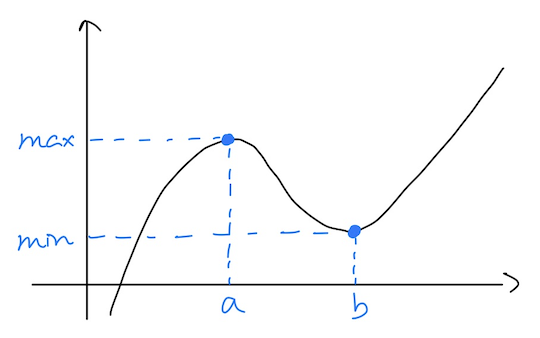
\includegraphics[scale=0.5]{Images/20.png}
}
\ex[]{$f: \bbR^2\to\bbR$}{
    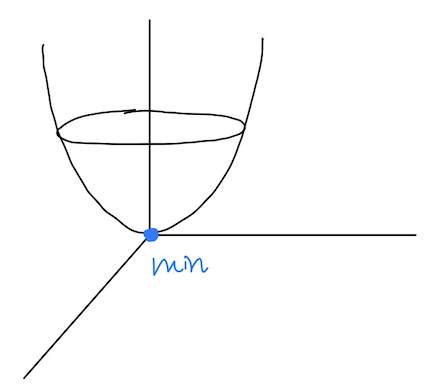
\includegraphics[scale=0.5]{Images/21.png}
}
Previously,
\begin{equation*}
    \begin{split}
        f: & \quad\bbR\to\bbR\\
        & \quad x\to x^3-x
    \end{split}
\end{equation*}
\begin{itemize}
    \item Find the domain: $D_f = \bbR$
    \item $f'(x) = 3x^2-1$
    \item Zeros of the first derivative: $f'(x)=0\Leftrightarrow x=\pm\frac{1}{\sqrt{3}} \to$ critical points
    \item Sign of $f'$ defines the monotony of $f$: $f'<0\to f$ is decreasing; $f'>0\to f$ is increasing
    \item $x=\frac{1}{\sqrt{3}}\to$ minimizer; $f(\frac{1}{\sqrt{3}})=-\frac{2\sqrt{3}}{3}\to$ minimum
    \item $x=-\frac{1}{\sqrt{3}}\to$ maximizer; $f(-\frac{1}{\sqrt{3}})=\frac{2\sqrt{3}}{3}\to$ maximum
\end{itemize}
\begin{center}
    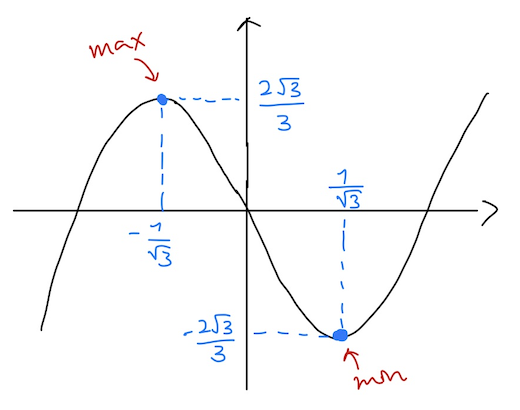
\includegraphics[scale=0.5]{Images/22.png}
\end{center}

If $f: u\to\bbR$ is a smooth map, it is not necessarily true that $f$ has a maximum or minimum.
However, if $f: K\to\bbR, K\subseteq\bbR^n$ where $K$ is compact, then $f$ has a maximum and minimum (\textbf{Weierstrass theorem}).

\section{Formal definition}
\dfn[]{Minimizer / Maximinzer}{
    If $f: u\to\bbR, u\subseteq\bbR^n, x_0\in u$.
    \begin{enumerate}
        \item We say that $x_o$ is a \textbf{global} minimizer of $f$ if $f(x_o)\leq f(x), \forall x\in u$
        \item We say that $x_o$ is a \textbf{local} minimizer of $f$ if there exists a neighborhood of $v$ such that $\forall x\in v, f(x_0)\leq f(x)$
    \end{enumerate}
    We can define analogously the global maximizer and local maximizer.
}
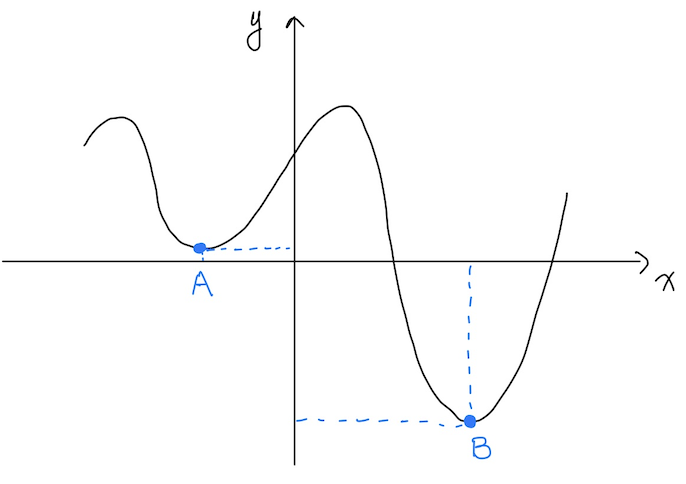
\includegraphics[scale=0.4]{Images/23.png} A is a local minimum and B is a global minimum.

\ex[]{Minimizer}{
    \noindent
    \begin{equation*}
        \begin{split}
            f: & \quad \bbR\to\bbR\\
            & \quad x\to 4x^2-4x+1
        \end{split}
    \end{equation*}
    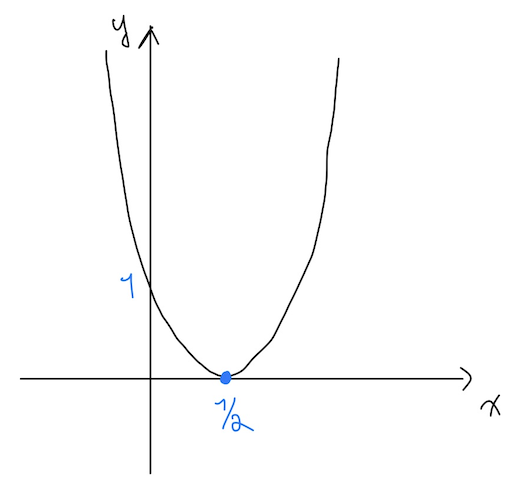
\includegraphics[scale=0.4]{Images/24.png}\\

    $\frac{1}{2}$ is a global minimizer\\
    $f(\frac{1}{2})=0$ is the minimum\\
    $f$ does not have a maximum
}
\ex[]{Maximizer}{
    \noindent
    \begin{equation*}
        \begin{split}
            f: & \quad \bbR^2\to\bbR\\
            & \quad (x,y)\to 1-x^2-y^2
        \end{split}
    \end{equation*}
    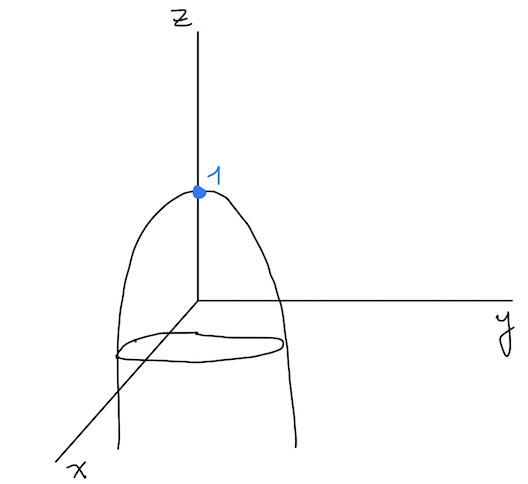
\includegraphics[scale=0.4]{Images/25.png}\\

    $(0,0)$ is the global maximizer\\
    1 is the global maximum
}

\section{Optimization: how to compute maximizer / minimizer?}
\begin{equation*}
    \begin{split}
        f: & \quad u\to\bbR, u\subseteq\bbR^n\\
        & \quad (x_1,\ldots,x_n)\to f(x_1,\ldots,x_n)
    \end{split}
\end{equation*}

\begin{equation*}
    \underbrace{\text{J}_f(x_1,\ldots,x_n)}_{\text{Jacobian Maxtrix}} = \left[\frac{\partial f}{\partial x_1}(x_1,\ldots,x_n) \cdots \frac{\partial f}{\partial x_n}(x_1,\ldots,x_n)\right]_{1\times n}
\end{equation*}

\textbf{Gradient} of $f$ is 
\begin{equation*}
    \nabla f(x_1,\ldots,x_n) = \left(\frac{\partial f}{\partial x_1}(x_1,\ldots,x_n) \cdots \frac{\partial f}{\partial x_n}(x_1,\ldots,x_n)\right)
\end{equation*}
and the \textbf{critical points} of $f$ are the zeros of $\nabla f(x_1,\ldots,x_n) \Leftrightarrow \nabla f(x_1,\ldots,x_n)=\vec{0}$

\ex[]{Critical point}{
    \noindent
    \begin{equation*}
        \begin{split}
            f: & \quad \bbR^2\to\bbR\\
            & \quad (x,y)\to 1-x^2-y^2
        \end{split}
    \end{equation*}

    Finding the gradient: $\nabla f(x_1,\ldots,x_n) = (-2x;-2y)$\\
    Finding the zeros of the gradient: $\nabla f(x_1,\ldots,x_n) = (0,0) \Leftrightarrow 
    \begin{cases}
        -2x = 0\\
        -2y = 0
    \end{cases} \Leftrightarrow
    \begin{cases}
        x = 0\\
        y= 0
    \end{cases}\\ \Rightarrow (0,0)$ is the unique crtical point of $f$ 
}

\textbf{Proposition:} Under the following conditions
\begin{itemize}
    \item $f: D_f\to\bbR, D_f\subseteq\bbR^n$
    \item $x_0\in\text{int}(D_f)$
\end{itemize}
If $x_0$ is an extremum (maximum or a minimum), then $x_0$ is a critical point.
\wc[]{The reverse of the proposition}{
    The reverse is not true. For example, $f(x) = x^3 \Rightarrow f'(x)=3x^2$. $f'(x)=0 \Leftrightarrow x=0$. $\{0\}$ is not a critical point but rather a saddle point.
}
The previous result gives \textbf{candidates} for maximizer or minimizer. Now, another question occers: how do we check that the critical point is a maximizer or minimizer?

\begin{gather*}
    f: \quad u\to\bbR, u\subseteq\bbR^n\\
    \nabla f(x_1,\ldots,x_n) = \left(\frac{\partial f}{\partial x_1}(x_1,\ldots,x_n) \cdots \frac{\partial f}{\partial x_n}(x_1,\ldots,x_n)\right)\\
    \underbrace{\text{H}_f(x_1,\ldots,x_n)}_{\text{Hessian Matrix}} = 
    \left[\begin{array}{cccc}
        \frac{\partial^2 f}{\partial x_1\partial x_1} & \frac{\partial^2 f}{\partial x_2\partial x_1} & \cdots & \frac{\partial^2 f}{\partial x_n\partial x_1}\\
        \vdots & \ddots & & \vdots\\
        \vdots & & \ddots & \vdots\\
        \frac{\partial^2 f}{\partial x_n\partial x_1} & \cdots & \cdots & \frac{\partial^2 f}{\partial x_n\partial x_n}
    \end{array}\right]_{n\times n}
\end{gather*}

\ex[]{Hessian matrix}{
    \noindent
    \begin{equation*}
        \begin{split}
            f: & \quad \bbR^2\to\bbR\\
            & \quad (x,y)\to 1-x^2-y^2
        \end{split}
    \end{equation*}\\
    $\nabla f(x,y) = (-2x, -2y)$\\

    $\text{H}_f(x,y) = 
    \left[
        \begin{array}{cc}
            -2 & 0\\
            0 & -2
        \end{array}
    \right]$
}
\thm[]{Schwarz theorem}{
    If $f$ is $C^2$, differentiable twice, then $\frac{\partial^2 f}{\partial x\partial y} = \frac{\partial^2 f}{\partial y\partial x}$.
}
In particular, the this result forces the Hessian matrix to be symmetric, $A^T = A$.
\begin{equation*}
    \text{H}_f(x_1,\ldots,x_n)^T = \text{H}_f(x_1,\ldots,x_n)
\end{equation*}
where $\text{H}_f$ defines a quadratic form.

\section{Quadratic forms in $\bbR^n$}
Sum of monomials of degree 2 in $\bbR^n$.
\pr[]{Is it a quadratic form?}{
    $\bbR: (x)$
    \begin{itemize}
        \item $P(x) = 7x^2 \to$ It is a quadratic form
        \item $Q(x) = 3 + 7x^2 \to$ Not a quadratic form because 3 is not of degree 2
    \end{itemize}
    $\bbR^2: (x,y)$
    \begin{itemize}
        \item $P(x) = 7x^2 + 8xy \to$ It is a quadratic form
        \item $Q(x) = 3^2x + y^2 \to$ Not a quadratic form because the first term is not of degree 2
    \end{itemize}
    $\bbR^3: (x,y,z)$
    \begin{itemize}
        \item $P(x) = 7x^2 + 8xy + \sqrt{2}y^2 \to$ It is a quadratic form
    \end{itemize}
}
To generalize, $\displaystyle\bbR^n(x_1,\ldots,x_n) : P(x_1,\ldots,x_n) = \sum_{i,j\in\{1,\ldots,n\}}c_{ij}x_ix_j$ is a quadratic form.\\

Associated to the quadratic form $Q$ in $\bbR^n$, we may define a matrix $A$ such that
\begin{equation}
    Q(x_1,\ldots,x_n) = [x_1\cdots x_n]A\left[\begin{array}{c}
        x_1\\
        \vdots\\
        x_n
    \end{array}\right], A\in \text{M}_{n\times n}(\bbR)
\end{equation}

\ex[]{A matrix}{
    $P(x,y) = 3x^2+8xy+5y^2$\\

    $P(x,y) = [x\quad y]\left[
        \begin{array}{cc}
            3 & 5\\
            3 & 5
        \end{array}
    \right]
    \left[\begin{array}{c}
        x\\
        y
    \end{array}\right]$\\

    $P(x,y) = [x\quad y]\left[
        \begin{array}{cc}
            3 & 8\\
            0 & 5
        \end{array}
    \right]
    \left[\begin{array}{c}
        x\\
        y
    \end{array}\right]$
}
There are infinitely many matrices $A$ such that equation (2.1) holds. However, just one is symmetric. For the previous example
\begin{equation*}
    P(x,y) = [x\quad y]\left[
        \begin{array}{cc}
            3 & 4\\
            4 & 5
        \end{array}
    \right]
    \left[\begin{array}{c}
        x\\
        y
    \end{array}\right]
\end{equation*}
Trick is to put the coefficient of the squared terms on the diagonal and the coefficient divided by two for the cross terms to fill in the rest of the matrix.
\pr[]{What is the symmatric matrix $A$?}{
    $P(x,y,z) = x^2 + 8xy - y^2 - 3xz + 10z^2$\\

    $A 
    = \left[\begin{array}{ccc}
        x^2 & xy & xz\\
        yx & y^2 & yz\\
        zx & zy & z^2
    \end{array}\right]
    = \left[\begin{array}{ccc}
        1 & 4 & -\frac{3}{2}\\
        4 & -1 & 0\\
        -\frac{3}{2} & 0 & 10
    \end{array}\right]$
}

\subsection{Classification of quadratic forms in $\bbR^n$}
$Q : $ a quadratic form
\dfn[]{$Q$ classifications}{
    \begin{enumerate}
        \item $Q$ is positively defined (P.D.) if $\,\forall x\in\bbR^n\textbackslash\{\vec{0}\}\quad Q(x)>0$
        \item $Q$ is negatively defined (N.D.) if $\,\forall x\in\bbR^n\textbackslash\{\vec{0}\}\quad Q(x)<0$
        \item $Q$ is semi-positively defined (S.P.D.) if $\,\forall x\in\bbR^n\quad Q(x)\geq0\quad\exists y\in\bbR^n\textbackslash\{\vec{0}\} : Q(y) = 0$
        \item $Q$ is semi-negatively defined (S.N.D) if $\,\forall x\in\bbR^n\quad Q(x)\leq0\quad\exists y\in\bbR^n\textbackslash\{\vec{0}\} : Q(y) = 0$
        \item $Q$ is undefined (UND.) if $\,\exists x,y\in\bbR^n : Q(x)=0, \,Q(y) = 0$
    \end{enumerate}
}
\ex[]{$Q$ classifications}{
    \begin{enumerate}
        \item $Q(x,y) = x^2+3y^2 \to$ is P.D.
        \item $Q(x,y) = -3x^2-7y^2 \to$ is N.D.
        \item $Q(x,y) = \underbrace{(x-y)^2}_{\geq 0} \to$ is S.P.D. since $Q(1,1) = 0$
        \item $Q(x,y) = -(7x-y)^2 \to$ is S.N.D.
        \item $Q(x,y) = x^2-y^2 \to$ is UND. since $Q(1,0) = 1$ and $Q(0,1)=-1$
    \end{enumerate}
}
In general, just by observing the quadratic forms is difficult to classify. We are going to establish two criteria to help us.\\

Let $A$ be the symmetric matrix associated to $Q$ and let $\lambda_1,\ldots,\lambda_n$ be the eigenvalues associated to $A$.
\thm[]{Classification using eigenvalues}{
    \begin{enumerate}
        \item $\lambda_1>0,\ldots,\lambda_n>0 \Rightarrow Q$ is P.D.
        \item $\lambda_1<0,\ldots,\lambda_n<0 \Rightarrow Q$ is N.D.
        \item $\lambda_1=0, \lambda_2>0,\ldots,\lambda_n>0 \Rightarrow Q$ is S.P.D
        \item $\lambda_1=0, \lambda_2<0,\ldots,\lambda_n<0 \Rightarrow Q$ is S.N.D
        \item $\exists i,j : \lambda_i>0, \lambda_j<0 \Rightarrow Q$ is UND.
    \end{enumerate}
}
\textbf{Remark: }To find the eigenvalues
\begin{itemize}
    \item $A\in M_{n\times n}(\bbR)$
    \item $\exists v\neq\bbR^n : Av = \lambda v$
    \item $\vec{v} \to$ eigenvector
    \item $\lambda\to$ eigenvalues
    \item $\lambda$ eigenvalues iff $P(\lambda)=0 \to \det(A-\lambda\,\text{I}_n)$
\end{itemize}
\pr[]{What is the eigenvector?}{
    $A = \left[\begin{array}{ccc}
        1 & 2 & 0\\
        2 & 4 & 0\\
        0 & 0 & 7
    \end{array}\right]$
    \begin{align*}
        P(\lambda) & = \det(A-\lambda I_d)\\
        & = \left|\begin{array}{ccc}
            1-\lambda & 2 & 0\\
            2 & 4-\lambda & 0\\
            0 & 0 & 7-\lambda
        \end{array}\right|\\
        & = (7-\lambda)\left|\begin{array}{cc}
            1-\lambda & 2\\
            2 & 4-\lambda
        \end{array}\right|\\
        & = (7-\lambda)[(1-\lambda)(4-\lambda)-4]\\
        & = (7-\lambda)(4-\lambda-4\lambda+\lambda^2-4)\\
        & = (7-\lambda)\underbrace{(\lambda^2-5\lambda)}_{\lambda(\lambda-5)}
    \end{align*}
    $\Rightarrow \lambda = 7 \land \lambda = 0 \land \lambda = 5$\\

    Choosing $\lambda = 7$\\
    \begin{align*}
        A\left[\begin{array}{c}
            x\\
            y\\
            z
        \end{array}\right] & = 7\left[\begin{array}{c}
            x\\
            y\\
            z
        \end{array}\right]\Leftrightarrow\\
        (A-\lambda I_d)\left[\begin{array}{c}
            x\\
            y\\
            z
        \end{array}\right] & = \vec{0} \Leftrightarrow\\
        \left[\begin{array}{ccc}
            -6 & 2 & 0\\
            2 & -3 & 0\\
            0 & 0 & 0
        \end{array}\right]\left[\begin{array}{c}
            x\\
            y\\
            z
        \end{array}\right] & = \left[\begin{array}{c}
            0\\
            0\\
            0
        \end{array}\right] \Leftrightarrow\\
        \begin{cases*}
            -6x+2y = 0\\
            2x - 3y = 0\\
            z \in \bbR
        \end{cases*} & \Leftrightarrow \begin{cases*}
            x = 0\\
            y = 0\\
            z \in \bbR
        \end{cases*}
    \end{align*}
    $\Rightarrow E_7 = \langle(0,0,\bbR)\rangle$
}
\ex[]{Classification using eigenvalues}{
    \begin{enumerate}
        \item $Q(x,y) = x^2+3y^2$\\
        
            $A = \left[\begin{array}{cc}
                1 & 0\\
                0 & 3
            \end{array}\right]\rightarrow\lambda_1 = 1, \,\lambda_2 = 3\Rightarrow$ P.D.
        \item $Q(x,y) = -3x^2-7y^2$\\
        
            $A = \left[\begin{array}{cc}
                -3 & 0\\
                0 & -7
            \end{array}\right]\rightarrow\lambda_1 = -3, \,\lambda_2 = -7\Rightarrow$ N.D.
        \item $Q(x,y) = (x-y)^2$\\
            
            $A = \left[\begin{array}{cc}
                1 & -1\\
                -1 & 1
            \end{array}\right]$\\

            $P(\lambda)=\left|\begin{array}{cc}
                1-\lambda & -1\\
                -1 & 1-\lambda
            \end{array}\right|=(1-\lambda)^2-1=1-2\lambda+\lambda^2-1=\lambda(\lambda-2)\rightarrow\lambda_1 = 0, \,\lambda_2 = 2\Rightarrow$ S.P.D
        \item $Q(x,y) = -(7x-y)^2$\\
        
            $A = \left[\begin{array}{cc}
                -49 & 7\\
                7 & -1
            \end{array}\right]\rightarrow\lambda_1 = 0, \,\lambda_2 <0\Rightarrow$ S.N.D
        \item $Q(x,y) = x^2-y^2$\\
        
            $A = \left[\begin{array}{cc}
                1 & 0\\
                0 & -1
            \end{array}\right]\rightarrow\lambda_1 = 1, \,\lambda_2 =-1\Rightarrow$ UND.
    \end{enumerate}
}

Associated to a quadratic form $Q : \bbR^n\to\bbR$, we may define a unique symmetric matrix $A$.
\thm[]{Sylvestor's theorem: Leading Minors Method}{
    If $\det A\neq 0$ and
    \begin{itemize}
        \item $\triangle_1>0, \triangle_2>0, \triangle_3>0, \triangle_4>0,\ldots\Rightarrow Q$ is P.D.
        \item $\triangle_1<0, \triangle_2>0, \triangle_3<0, \triangle_4>0,\ldots\Rightarrow Q$ is N.D.
        \item $Q$ is undefined otherwise
    \end{itemize}
    
}
The leading minors are the determinants of each $\triangle_i$
\begin{center}
    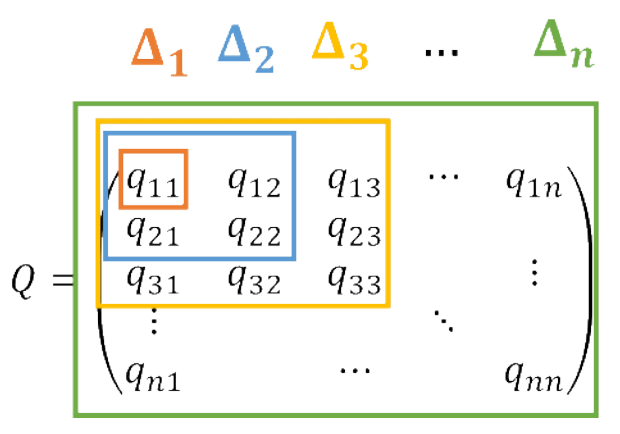
\includegraphics[scale=0.5]{Images/26.png}
\end{center}
\ex[]{Classification of $Q$ using all three methods}{
    \begin{enumerate}
        \item $Q(x,y) = x^2-y^2$
            \begin{itemize}
                \item Definition\\
                    $f(1,0) = 1 > 0$\\
                    $f(0,1) = -1 < 0$\\
                    $\Rightarrow$ UND.
                \item Eigenvalues\\
                    $A = \left[\begin{array}{cc}
                        1 & 0\\
                        0 & 1
                    \end{array}\right]$\\
                    $\lambda_1 = 1, \lambda_2 = -1 \Rightarrow$ UND.
                \item Sylvester's\\
                    $\triangle_1 = 1, \triangle_2 = -1 \Rightarrow$ UND.
            \end{itemize}
        \item $Q(x,y,z) = -x^2-2y^2-3z^2$
            \begin{itemize}
                \item Definition\\
                    All negative except at $\vec{0}\Rightarrow$ N.D.
                \item Eigenvalues\\
                    $A = \left[\begin{array}{ccc}
                        -1 & 0 & 0\\
                        0 & -2 & 0\\
                        0 & 0 & -3
                    \end{array}\right]$\\
                    $\lambda_1 = -1, \lambda_2 = -2, \lambda_3 = -3 \Rightarrow$ N.D.
                \item Sylvestor's\\
                    $\triangle_1 = -1, \triangle_2 = 2, \triangle_3 = -6 \Rightarrow$ N.D.
            \end{itemize}
    \end{enumerate}
}
\thm[]{Local minimizer / maximizer}{
    \begin{itemize}
        \item $f: u\to\bbR$
        \item $u \subseteq\bbR^n$ is open
        \item $\nabla f(x_0) = \vec{0},\, x_0\in\bbR^n$
    \end{itemize}
    If $H_f$ defines a P.D. quadratic form, then $x_0$ is a local minimizer.\\
    If $H_f$ defines a N.D. quandratic form, then $x_0$ is a local maximizer.
}

\dfn[]{Saddle point}{
    If $x_0$ is a critical point and $x_0$ is neither a maximizer nor a minimizer, then $x_0$ is a saddle point.
}
\ex[]{Local maximizer / minimizer}{
    \begin{enumerate}
        \item $f: \bbR \to \bbR \qquad x\to -(x+2)^2+3$\\

            $f'(x) = -2(x+2)$\\
            $f'(x) = 0 \Leftrightarrow x = -2 \Rightarrow -2$ is a critical point\\
            $f''(x) = -2 < 0 \Rightarrow$ is N.D.\\
            $\Rightarrow -2$ is a local maximizer.
        \item $f: \bbR^2 \to \bbR \qquad f(x,y) = x^2+3y^2$\\
        
            $J_f=\left[\begin{array}{cc}
                2x & 6y
            \end{array}\right] \rightarrow \nabla f(x,y) = (2x, 6y)$\\
            $\nabla f(x,y) = \vec{0} \Leftrightarrow \begin{cases*}
                2x = 0\\
                6y = 0
            \end{cases*} \Leftrightarrow \begin{cases*}
                x = 0\\
                y = 0
            \end{cases*}$\\
            $\therefore (0,0)$ is a critical point\\
            $H_f = \left[\begin{array}{cc}
                2 & 0\\
                0 & 6
            \end{array}\right] \Rightarrow \lambda_1 = 2, \lambda_2 = 6 \Rightarrow$ defines a P.D. quadratic form\\
            $(0,0)$ is a local minimizer.
    \end{enumerate}
}

Now we are going to check if a local extremum could be seen as a global extremum. For example, $f: \bbR\to\bbR$
\begin{center}
    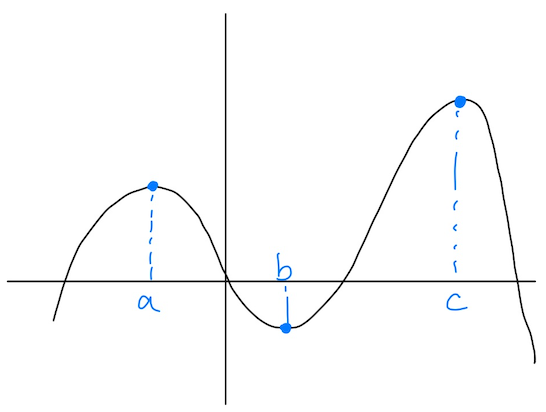
\includegraphics[scale=0.5]{Images/27.png}
\end{center}
c is a global maximizer because $f(c)$ is the maximum of the map. $f(x)\leq f(c)\, ,\forall x\in\bbR$.\\

We first need to establish the concept of \textbf{convexity} of the graph of a map. 
The graph of $f$ is convex if the line connecting any two points $A\hookrightarrow(a, f(a))$ and $B\hookrightarrow(b, f(b))$ is above the graph of $f$.
The graph of $f$ is concave if the line connecting any two points $A\hookrightarrow(a, f(a))$ and $B\hookrightarrow(b, f(b))$ is below the graph of $f$.
\begin{center}
    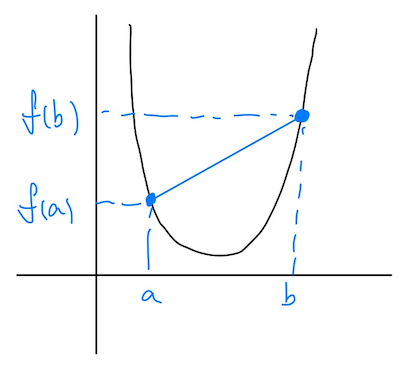
\includegraphics[scale=0.5]{Images/28.png}
    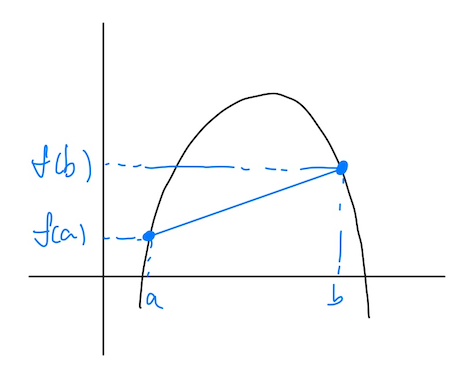
\includegraphics[scale=0.5]{Images/29.png}
\end{center}
We can extend the definition for maps defined in $\bbR^n$, above $\to$ inside and below $\to$ outside.

\dfn[]{Classification of $H_f$}{
    If $H_f$ defines a positvely defined quadratic form for all points $x\in\bbR^n$, then we say that $H_f$ is positive. 
    Analogous result for negative.
}
\thm[]{Global minimizer / maximizer}{
    $f: u\to\bbR\, ,u\subseteq \bbR^n\, ,u$ is open
    \begin{itemize}
        \item $H_f$ is positive $\Rightarrow$ graph of $f$ is convex $\Rightarrow$ any local minimizer is a global minimizer
        \item $H_f$ is negative $\Rightarrow$ graph of $f$ is concave $\Rightarrow$ any local maximizer is a global maximizer
    \end{itemize}
}

\section{Optimization with restrictions given by equalities}

Setting up the problem, we have a \textbf{map}
\begin{equation*}
    f: u\to\bbR, u\subseteq\bbR^n \quad\text{differentiable}
\end{equation*}
and we have the \textbf{restrictions}
\begin{equation*}
    \begin{cases*}
        g_1(x_1,\ldots,x_n) = 0\\
        g_2(x_1,\ldots,x_n) = 0\\
        \vdots\\
        g_k(x_1,\ldots,x_n) = 0
    \end{cases*}
\end{equation*}
with the \textbf{hypothesis} that rank[$g_1 \cdots g_k$] $\neq 0$, the restrictions are not linearly dependent. 
For example, $x^2 + y^2 = 1, x^2 + y^2 = 4$ are linearly dependent and the hypothesis avoides this type of situation.\\

The technique is
\begin{equation*}
    \mcL(x_1,\ldots,x_n,\lambda_1,\ldots,\lambda_p) = f(x_1,\ldots,x_n)-\lambda_1g_1(x_1,\ldots,x_n)-\cdots -\lambda_pg_p(x_1,\ldots,x_n)
\end{equation*}
where $\mcL$ is the Lagrangean map.

\thm[]{Lagrangean}{
    If $x^*$ is a minimum/maximum of $f$ with the restrictions $g_i(x) = 0, i=1,\ldots,p$,
    then $x_0$ is a solution of
    \begin{equation*}
        \nabla\mcL(x_1,\ldots,x_n,\lambda_1,\ldots,\lambda_p) = \vec{0}
    \end{equation*}
    where $\lambda_1,\ldots,\lambda_p$ are the Lagrange multipliers.
}
Do not forget that the problem has a solution if the hypothesis holds.

\ex[]{Lagrangean}{
    \noindent
    \begin{equation*}
        \begin{split}
            f: & \quad \bbR^2\to\bbR\\
            & \quad (x,y)\to xy
        \end{split}
    \end{equation*}
    with the restriction $x^2+y^2=2$\\

    We have one restriction: $g_1(x,y) = x^2+y^2-2 = 0$\\
    \begin{equation*}
        \mcL(x,y,\lambda) = xy - \lambda(x^2+y^2-2)
    \end{equation*}
    \begin{align*}
        \nabla\mcL(x,y,\lambda) & = \left(\frac{\partial\mcL}{\partial x}, \frac{\partial\mcL}{\partial y}, \frac{\partial\mcL}{\partial \lambda}\right)\\
        & = (y-2\lambda x, x-2\lambda y, -(x^2+y^2-2))
    \end{align*}
    \begin{equation*}
        \nabla\mcL(x,y,\lambda) = \vec{0} \Leftrightarrow
        \begin{cases*}
            y - \lambda 2x = 0\\
            x - \lambda 2y = 0\\
            -(x^2+y^2-2) = 0
        \end{cases*}
    \end{equation*}
    Now solving the system of equations.\\

    From the first two equations, we have $y = 2\lambda x$ and $x = 2\lambda y$. Replacing $y$ in the second equation
    \begin{equation*}
        x = 2\lambda(2\lambda x) \Rightarrow x(1-4\lambda^2) = 0 \Rightarrow \begin{cases*}
            x = 0\\
            \lambda = \pm\frac{1}{2}
        \end{cases*}
    \end{equation*}
    \begin{itemize}
        \item If $x=0$, then then we have $y=0$ from the first equation. But this contradicts the restriction $x^2+y^2=2$. So, no critical point in this case.
        \item If $\lambda = \frac{1}{2}$, then from the first equation $y = x$. Replacing in the restriction $x^2+x^2=2 \Rightarrow x = \pm 1 \Rightarrow y = \pm 1$. So, we have two critical points $(1,1)$ and $(-1,-1)$.
        \item If $\lambda = -\frac{1}{2}$, then from the first equation $y = -x$. Replacing in the restriction $x^2+(-x)^2=2 \Rightarrow x = \pm 1 \Rightarrow y = \mp 1$. So, we have two critical points $(1,-1)$ and $(-1,1)$.
    \end{itemize}
    $\Rightarrow$ The critical points are $(1,1), (-1,-1), (1,-1), (-1,1)$\\
    
    Now we have to classify the critical points. Evaluating $f$ at each critical point,
    \begin{itemize}
        \item $f(1,1) = 1\rightarrow$ maximum
        \item $f(-1,-1) = 1\rightarrow$ maximum
        \item $f(1,-1) = -1\rightarrow$ minimum
        \item $f(-1,1) = -1\rightarrow$ minimum
    \end{itemize}
}

%\dfn{Definition Topic}{Definition Statement}
%\thm{Theorem Name}{Theorem Statement}
%\cor[cori]{Corollary Name}{Corollary Statement}
%\lem{Lemma Name}{Lemma Statement}
%\clm{Claim Name}{Claim Statement}
%\ex{Example Name}{Example explained}
%\opn{Open Question Name}{Question Statement}
%\pr{Question Name}{Question Statement}
%\nt{Special Note}
%\wc{Wrong Concept topic}{Explanation}
%\proof{Proof Idea}{}